\chapter{Statica}
L'obiettivo della statica è quello di determinare la relazione tra:
\begin{itemize}
	\item Il \emph{wrench di forza} applicato dall'organo terminale sull'ambiente esterno,
	\begin{equation}
		\underline{\gamma} = 
		\begin{bmatrix}
			\underline{f} \\
			\underline{\mu} \\
		\end{bmatrix}
	\end{equation} con $\underline{f}$ la forza risultante e $\underline{\mu}$ il momento risultante attorno all'origine della terna utensile.
	\item Le \emph{azioni generalizzate} $\underline{\tau}$ che gli attuatori devono esercitare sui giunti per equilibrare $\underline{\gamma}$. Queste azioni posso essere \emph{coppie} se si tratta di giunti rotoidali o \emph{forze} se si tratta di giunti prismatici. Notiamo che \emph{non} equilibra eventuali azioni dinamiche e nemmeno azioni gravitazionali come il peso dei link.
\end{itemize}

In pratica, vogliamo sapere quali coppie generalizzate (forze) devono essere applicate sui giunti (degli attuatori) affinché \emph{l'E-E} (End Effector) eserciti sull'ambiente un \emph{wrench} assegnato $\underline{\gamma}$.
\section{Principio dei Lavori Virtuali}
Per trovare la relazione tra $\underline{\gamma}$ e $\underline{\tau}$ utilizziamo il \emph{principio dei lavori virtuali} (PLV). Esso affermo che:

\textit{in un sistema meccanico in equilibrio, il lavoro $\delta W$ fatto da tutte le forze e coppie agenti sul sistema in conseguenza di un qualsiasi spostamento virtuale $\delta \underline{q}$ è nullo,} ovvero:
\begin{equation}
	\delta W = 0
\end{equation}
uno spostamento virtuale è un piccolo cambiamento di configurazione $\delta \underline{q}$ compatibile con i vincoli esistenti. 

In generale, $\delta \underline{q} \neq d\underline{q}$, perchè non sempre uno spostamento elementare $d\underline{q}$ del sistema è compatibile con i vincoli esistenti. Ma nel caso di un robot a base fissa, tutte le componenti di uno spostamento virtuale sono indipendenti e pertanto un qualsiasi spostamento elementare arbitrario $d\underline{q}$ è anche uno spostamento virtuale $\delta \underline{q}$.

\paragraph{}
Le \textbf{azioni} (forze o coppie) che compiono lavoro in conseguenza di uno spostamento virtuale del robot $\delta \underline{q} = d\underline{q}$ sono:
\begin{itemize}
	\item Le azioni $\underline{\tau}$ degli attuatori sui giunti, i quali subiscono uno spostamento $d \underline{q}$.
	\item Il \emph{wrench} di forza pari a $-\gamma$ applicato sull'organo terminale, perchè se $\gamma$ è l'azione del manipolatore sull'ambiente, allora per il principio di azione e reazione, $-\gamma$ è l'azione dell'ambiente sul manipolatore.
\end{itemize}

\paragraph{}
Il \emph{lavoro virtuale} delle azioni $\underline{\tau}$ vale:
\begin{equation}
	\delta W_{\underline{\tau}} = \sum_{i = 1}^n \tau_i \delta q_i = \underline{\tau}^T \delta \underline{q}
\end{equation}

\paragraph{}
Il \emph{lavoro virtuale} delle azioni $-\underline{\gamma}$ vale:
\begin{equation*}
	\delta W_{- \underline{\gamma}} = \delta W_{- \underline{f}} + \delta W_{- \underline{\mu}} = - \underline{f}^T \delta \underline{p} - \underline{\mu}^T \underline{\omega} \delta t =
\end{equation*}
\begin{equation}
	= - \underline{f}^T J_p \delta \underline{q} - \underline{\mu}^T J_o \underbrace{\underline{\dot{q}} \delta t}_{\delta \underline{q}}  
\end{equation}

\paragraph{}
Il \emph{lavoro virtuale complessivo} risulta essere:
\begin{equation}
	\delta W = \delta W_{\underline{\tau}} + \delta W_{- \underline{\gamma}} = \delta W_{\underline{\tau}} + \delta W_{- \underline{f}} + \delta W_{- \underline{\mu}} = 0
\end{equation}
pertanto, 
\begin{equation}
	\underline{\tau}^T \delta \underline{q} - \underline{f}^T J_p \delta \underline{q} - \mu^T J_o \delta \underline{q} = \delta \underline{q} ( \underline{\tau}^T - \underline{f}^T J_p - \underline{\mu}^T J_o) = 0
\end{equation}
e otteniamo
\begin{equation}
	\delta \underline{q} \Biggl( \underline{\tau}^T - 
	\begin{bmatrix}
		\underline{f}^T & \underline{\mu}^T
	\end{bmatrix}
	\begin{bmatrix}
		J_p \\
		J_o \\
	\end{bmatrix}
    \Biggr) = \delta \underline{q} \Bigl( \underline{\tau}^T - \underline{\gamma}^TJ \Bigr) = 0 \; \Rightarrow \; \underline{\tau}^T - \underline{\gamma}^T J = 0
\end{equation}
quindi,
\begin{equation}
	\underline{\tau} = J^T \underline{\gamma} \quad \forall \delta \underline{q}
\end{equation}

\section{Dualità Cinetostatica}
La relazione statica ($6.8$), combinata con la relazione cinematica differenziale ($4.12$), mette in luce una proprietà di \emph{dualità cineto-statica}. Infatti, considerando la seguente rappresentazione 

\begin{center}
	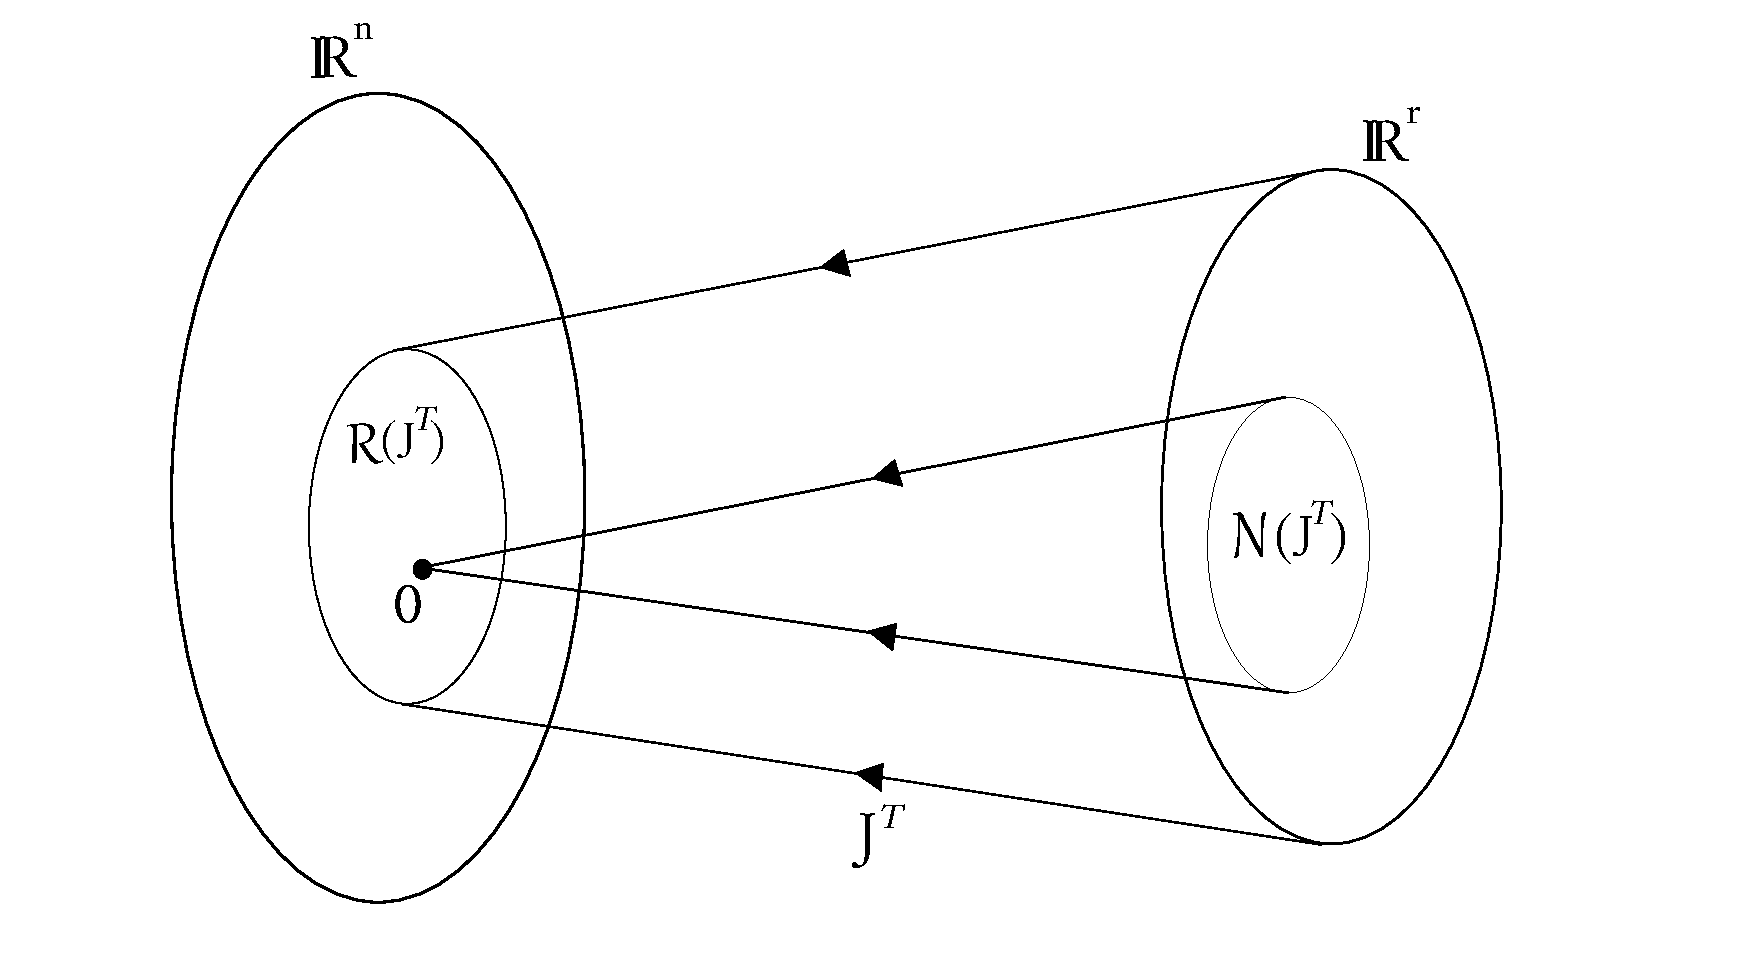
\includegraphics[scale=0.35]{dualitaCinetostatica.pdf}
	\caption{Relazione tra spazio delle forze all'organo terminale e spazio delle coppie ai giunti.}
\end{center}

si ottiene che:
\begin{itemize}
	\item L'immagine di $J^T$ è il sottospazio $\mathcal{R}(J^T)$ in $\mathbb{R}^n$ che individua le coppie ai giunti che possono bilanciare le forze all'organo terminale, nella configurazione assegnata al manipolatore.
	\item Il nullo di $J^T$ è il sottospazio $\mathcal{N}(J^T)$ in $\mathbb{R}^r$ a cui appartengono le forze all'organo terminale che non richiedono alcuna coppia di bilanciamento ai giunti, nella configurazione assegnata al manipolatore.
\end{itemize}
Notiamo che le forze all'organo terminale $\underline{\gamma} \in \mathcal{N}(J^T)$ sono interamente assorbite dalla struttura, nel senso che le reazioni vincolari sono in grado di bilanciarle esattamente.

\subsubsection{Relazione $\mathcal{N}(J^T) \perp \mathcal{R}(J)$}
La relazione tra i diversi sottospazi sono regolate da:
\begin{equation}
	\mathcal{N}(J) = \mathcal{R}^{\perp}(J^T) \qquad \mathcal{R}(J) = \mathcal{N}^{\perp}(J^T)
\end{equation}
ovvero, i due sottospazi sono legati dall'operazione di \emph{complemento ortogonale}. Dimostriamo questo legame procedendo per \emph{assurdo}:
\paragraph{}
\textit{
Sia $\underline{y}_{\,1} \in \mathcal{R}(J)$, $\underline{y}_{\,2} \in \mathcal{N}(J^T)$, con $\underline{y}_{\,1} = J \underline{\dot{q}}_{\,1}$. Supponiamo che $\underline{y}_{\,1}$ e $\underline{y}_{\,2}$ non siano ortogonali, ovvero che
\begin{equation}
	\underline{y}_{\,1}^T \underline{y}_{\,2} \neq 0
\end{equation} 
ma sappiamo che 
\begin{equation}
	\underline{y}_{\,1}^T \underline{y}_{\,2} = \underline{\dot{q}}_{\,1}^T J^T \underline{y}_{\,2}
\end{equation}
pertanto, dovrebbe valere $\underline{\dot{q}}_{\,1}^T J^T \underline{y}_{\,2} \neq 0$, e ciò significa che 
\begin{equation}
	J^T \underline{y}_{\,2} \neq 0
\end{equation}
e sapendo che $\underline{y}_{\,2} \in \mathcal{N}(J^T)$ la relazione ($6.12$) risulta impossibile, ed ecco l'assurdo.}